%%%%%%%%%%%%%%%%%%%%%%%%%%%%%%%%%%%%%%%%%%%%%%%%%%%%%%%%%%%%%%%%%%%%%%%%%%%%%%%%%%
\begin{frame}[fragile]\frametitle{}
\begin{center}
{\Large Integration}
\end{center}
\end{frame}

%%%%%%%%%%%%%%%%%%%%%%%%%%%%%%%%%%%%%%%%%%%%%%%%%%%%%%%%%%%
 \begin{frame}[fragile] \frametitle{Integration}


\begin{itemize}
\item Finding area under curve is done using Integration
\item It can be thought of OPPOSITE of Derivation.
\end{itemize}
\begin{center}
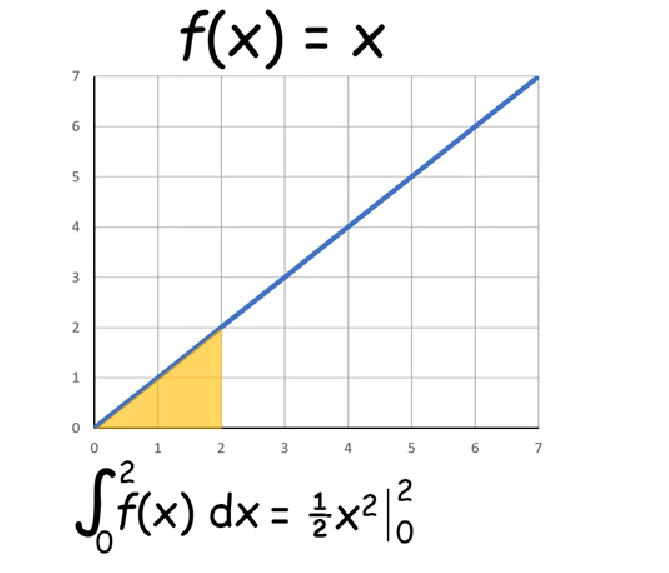
\includegraphics[width=0.5\linewidth,keepaspectratio]{intg1}
\end{center}

\end{frame}


%%%%%%%%%%%%%%%%%%%%%%%%%%%%%%%%%%%%%%%%%%%%%%%%%%%%%%%%%%%
 \begin{frame}[fragile] \frametitle{Integration}
What is the area under the curve of the function  $3x^2 + 2x + 1$  between 0  and  3 ?

\begin{lstlisting}
import numpy as np
from matplotlib import pyplot as plt
from matplotlib.patches import Polygon
%matplotlib inline

# Define function g
def g(x):
    return 3 * x**2 + 2 * x + 1

# Create an array of x values from 0 to 10
x = range(0, 11)

# Get the corresponding y values from the function
y = [g(a) for a in x]
\end{lstlisting}


\end{frame}

%%%%%%%%%%%%%%%%%%%%%%%%%%%%%%%%%%%%%%%%%%%%%%%%%%%%%%%%%%%
 \begin{frame}[fragile] \frametitle{Integration}
What is the area under the curve of the function  $3x^2 + 2x + 1$  between 0  and  3 ?

\begin{lstlisting}
# Set up the plot
fig, ax = plt.subplots()
plt.xlabel('x')
plt.ylabel('f(x)')
plt.grid()

# Plot x against g(x)
plt.plot(x,y, color='purple')

# Make the shaded region
ix = np.linspace(0, 3)
iy = g(ix)
verts = [(0, 0)] + list(zip(ix, iy)) + [(3, 0)]
poly = Polygon(verts, facecolor='orange')
ax.add_patch(poly)

plt.show()
\end{lstlisting}


\end{frame}

%%%%%%%%%%%%%%%%%%%%%%%%%%%%%%%%%%%%%%%%%%%%%%%%%%%%%%%%%%%
 \begin{frame}[fragile] \frametitle{Integration}

\begin{center}
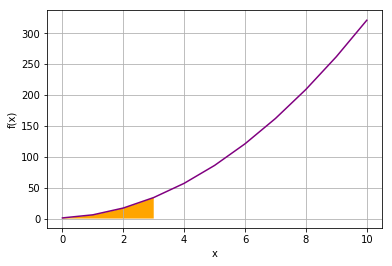
\includegraphics[width=0.5\linewidth,keepaspectratio]{intg2}
\end{center}

\end{frame}

%%%%%%%%%%%%%%%%%%%%%%%%%%%%%%%%%%%%%%%%%%%%%%%%%%%%%%%%%%%
 \begin{frame}[fragile] \frametitle{Integration}


$\int_0^3 3x^2 + 2x + 1\;dx$

The antiderivative of $3x^2 + 2x + 1\;dx$ is $\frac{3}{3} x^3 + \frac{2}{2} x^2 + x$, so


\begin{align}
\int_0^3= \frac{3}{3} x^3 + \frac{2}{2} x^2 + x\ \big|_0^3\\
= \frac{3}{3} 3^3 + \frac{2}{2} 3^2 + 3 - \frac{3}{3} 0^3 - \frac{2}{2} 0^2 + 0\\
= 27 + 9 + 3 + 0 + 0 + 0\\
= 39
\end{align}



\end{frame}